\documentclass[a4paper,12pt]{report}

% Encodage et langue
\usepackage[utf8]{inputenc}
\usepackage[T1]{fontenc}
\usepackage[french]{babel}
\usepackage{unicode-math}
\usepackage{amssymb}



% Mise en page
\usepackage{geometry}
\geometry{margin=2.5cm}

% Packages utiles
\usepackage{graphicx}  % Pour les images
\graphicspath{{images/}}

\usepackage{amsmath, amssymb}  % Pour les maths
\usepackage[hidelinks]{hyperref}  % Pour les liens
\usepackage{float}  % Pour le placement des figures

\usepackage{enumitem} 

\DeclareUnicodeCharacter{2260}{\neq}


\title{ Introduction au Data Mining}
\author{DNJOMOU YONMBA WILFRIED LOIC CM-UDS-24SCI0999 \\
KENFACK LEONEL CM-UDS-17SCI0998\\
SAGUEU WAKAM DILANE CM-UDS-24SCI1040\\}
\date{Mars 2024}

\begin{document}

\maketitle

\renewcommand{\contentsname}{Table des matières}

\tableofcontents

\renewcommand{\chaptername}{Chapitre}

\chapter*{Introduction Générale}
	À l’ère du numérique, la quantité de données générées croît de manière exponentielle, posant des défis mais offrant également des opportunités considérables. Le \textbf{Data Mining}, ou exploration de données, est une discipline qui permet d’extraire des informations pertinentes et exploitables à partir de vastes ensembles de données. Il se distingue d’autres domaines connexes tels que le \textbf{Big Data}, qui se concentre sur le stockage et la gestion des données massives, le \textbf{Machine Learning}, qui vise à créer des modèles prédictifs, et la \textbf{Business Intelligence}, orientée vers l’analyse et la visualisation des informations pour faciliter la prise de décision. L’objectif principal du Data Mining est la découverte de connaissances enfouies dans les données, afin de détecter des motifs cachés, d’optimiser la prise de décision et d’anticiper des tendances. Son essor est motivé par plusieurs facteurs, notamment l’explosion des données numériques, l’amélioration des capacités de calcul et le besoin croissant d’automatiser l’analyse d’informations complexes pour améliorer la productivité dans divers secteurs. Les applications du Data Mining sont vastes et couvrent de nombreux domaines : en santé, il permet la détection précoce de maladies ; en finance, il aide à l’évaluation des risques et à la détection de fraudes ; en marketing, il optimise les recommandations personnalisées ; en cybersécurité, il identifie les activités suspectes ; et en agriculture, il contribue à la gestion des cultures et des rendements. Dans la suite de notre travail, nous explorerons d’abord les principes fondamentaux et les enjeux du Data Mining. Nous détaillerons ensuite les \textbf{étapes de sa mise en œuvre}, les \textbf{techniques et algorithmes utilisés}, les outils et langages de programmation les plus répandus, avant d’aborder \textbf{ses limites et défis}, notamment ceux liés à la qualité des données, aux coûts de calcul et aux questions éthiques et de confidentialité. Cette analyse permettra de mieux comprendre l’impact du Data Mining dans un monde de plus en plus orienté vers la donnée.
\newpage

\chapter{Définition et Enjeux du Data Mining}
\textbf{Le data mining}, ou \textit{exploration de données}, consiste à analyser de grands ensembles de \textbf{données} pour découvrir des \textbf{modèles} et des \textbf{tendances cachés,} aidant ainsi les entreprises à résoudre des problèmes, atténuer des risques et identifier de nouvelles opportunités commerciales.

Avant d’aller plus en détail sur ce qu’est le data mining, commençons par définir ce qu’est une donnée (\textit{data}). \\


    \section{C'est quoi une donnée ?}
        Dans le contexte du data mining, \textbf{une donnée} représente une unité d'information brute collectée à partir de diverses sources. Ces données peuvent être de différentes natures, telles que des chiffres, du texte, des images ou des enregistrements audio. Elles sont généralement stockées dans des bases de données et servent de matière première pour l'analyse. Le data mining exploite ces données pour identifier des modèles, des tendances ou des relations cachées, fournissant ainsi des informations précieuses pour la prise de décision.\\

        En data mining, les données sont classées en trois catégories principales : \textit{structurées, semi-structurées et non structurées}. \\

        \subsection{Données Structurées}
            \textbf{Les données structurées} sont organisées selon un format prédéfini, généralement sous forme de tableaux avec des lignes et des colonnes. Chaque champ possède un type de données spécifique, facilitant le stockage, la recherche et l'analyse.\\

            \textbf{Exemples :}
            \begin{itemize}
                \item \textit{Bases de données relationnelles} contenant des informations clients (nom, adresse, numéro de téléphone).
                \item \textit{Feuilles de calcul} avec des données financières.
            \end{itemize}
            
            \textbf{Caractéristiques :}
            \begin{itemize}
                \item \textit{Organisation rigoureuse} avec un schéma fixe.
                \item Facilité d'accès et d'analyse grâce à des requêtes SQL.
                \item \textit{Moins flexible} en termes de modifications de structure.
            \end{itemize}\\


        \subsection{Données non structurées}
            \textbf{Les données non structurées} n'ont pas de format ou de modèle prédéfini, ce qui les rend plus complexes à collecter, traiter et analyser. Elles représentent la majorité des données disponibles et peuvent contenir des informations précieuses une fois correctement exploitées.\\

            \textbf{Exemples :}
            \begin{itemize}
                \item \textit{Documents texte} tels que des rapports ou des articles.
                \item \textit{Contenus multimédias} comme des images, vidéos et fichiers audio.
                \item \textit{Publications sur les réseaux sociaux ou messages instantanés.}
            \end{itemize}
            
            \textbf{Caractéristiques :}
            \begin{itemize}
                \item \textit{Absence de structure formelle}, rendant l'analyse plus complexe.
                \item \textit{Nécessite des techniques avancées} telles que le traitement du langage naturel ou la reconnaissance d'images pour extraire des informations pertinentes.
            \end{itemize}\\

        \subsection{Données semi-structurées}
            \textbf{Les données semi-structurées} ne suivent pas un schéma strict, mais possèdent des balises ou des marqueurs pour séparer les éléments de données. Elles combinent des aspects des données structurées et non structurées, offrant une certaine organisation sans la rigidité des bases de données relationnelles.\\

            \textbf{Exemples :}
            \begin{itemize}
                \item \textit{Fichiers XML ou JSON} utilisés pour échanger des données entre systèmes.
                \item \textit{Emails contenant des métadonnée}s (expéditeur, destinataire) et du contenu libre.
            \end{itemize}
            
            \textbf{Caractéristiques }:
            \begin{itemize}
                \item \textit{Flexibilité accrue} par rapport aux données structurées.
                \item \textit{Nécessite des outils spécifiques pour l'analyse}, capables de comprendre la structure implicite.
            \end{itemize}

            Il est important de noter qu’il existe plusieurs autres classification de la données. Par exemple, on peut les classer selon la nature de leur variables. \\

        \subsection{Nature des variables}    
            \textbf{Une variable} - une colonne d'une table, attribut ou champ -, contient deux types de données : \textit{les données qualitatives et les données quantitatives}.\\

            \textbf{Une données qualitative} exprime une qualité, c'est-à-dire un statut unique et est de nature discrète : les valeurs peuvent être listées et répétées pour plusieurs enregistrements. \\ 
            
            Prenons l'exemple de la couleur des yeux. Les valeurs peuvent être listées   (bleu, vert, marron, noisette, ambre ), et la même valeur pourrait être répétée pour plusieurs individus.
            On distingue : 
            \begin{itemize}
                \item \textbf{Variable qualitative ordinale:} les valeurs peuvent être organisées selon une certaine hiérarchie.\\
                \textbf{Exemple :} \textit{Grand, Moyen, Petit}.
                \item \textbf{Variable qualitative nominale:}  les valeurs ne peuvent pas être organisées selon une certaine hiérarchie. \\
                \textbf{Exemple :} \textit{bleu, vert, jaune.}
            \end{itemize}\\
            
           \textbf{Une variable quantitative} contient des valeurs numériques - qui peuvent être mesurées ou agrégées ( que l'on peut quantifier ). Nous retrouvons comme exemple la taille, le poids, le revenu, l'âge, la température,...
            Une variable quantitative est également dissociée en deux sous-catégories :
            
            \begin{itemize}
                \item \textbf{Variable quantitative proportionnelle:} les différences entre les valeurs peuvent être caractérisées par des proportions égales de sorte qu'il existe une relation mathématique et constante. \\
                \textbf{Exemple :} Une personne qui pèse 90kg est deux fois plus lourde qu’une personne qui pèse 45 kg.
                \item \textbf{Variable quantitative intervalle:} les intervalles entre les valeurs ne sont pas constants. \\
                \textbf{Exemple :} mesure de la température – 15/12/2024 13:45:34 7,2 C° ; 15/12/2024 13:46:15 7,1 C° ; 15/12/2024 13:52:55 7,4 C°.
            \end{itemize}\\
            
        Comprendre ces différents types de données est essentiel en data mining, car chaque catégorie nécessite des approches et des outils spécifiques pour être efficacement exploitée et transformer les données brutes en informations utiles. \\
        
        Maintenant que nous savons ce qu’est une donnée et que nous savons distinguer les différents types, voyons maintenant ce qu’est le data mining plus en détail !
    

    \section{Data mining : Définition et Enjeux}
        \textbf{Le data mining}, ou \textit{exploration de données} ou encore \textit{forage de données}, est le processus d'analyse de grands volumes de données du big data pour découvrir des modèles et des tendances cachés. 

        Il utilise des techniques sophistiquées issues de la \textbf{statistique}, et de \textbf{l'intelligence artificielle} pour analyser en profondeur des données sous différents angles afin de tirer des informations utiles. Ces informations peuvent ensuite être utilisées par les entreprises pour augmenter un chiffre d’affaires ou pour réduire des coûts.
        Grâce à l'exploration de données, les entreprises peuvent faire face à diverses situations.  

        \subsection{Prédire et anticiper les tendances}
            En analysant les données passées, le Data mining permet de détecter des schémas et des tendances, ce qui aide les entreprises à anticiper les comportements futurs des clients, des marchés ou des produits. 
            Par exemple, une entreprise qui commercialise des produits peut utiliser le Data mining pour prédire les produits qui seront les plus populaires lors de certaines saisons ou événements.
        
        \subsection{Optimisation des processus internes}
            En identifiant les inefficacités et les opportunités d'amélioration dans les processus commerciaux, l'exploration de données permet aux entreprises de prendre des décisions plus éclairées pour optimiser leurs opérations. 
            Par exemple, une entreprise de fabrication peut utiliser l'exploration de données pour identifier les goulots d'étranglement dans sa chaîne d'approvisionnement et les résoudre pour améliorer l'efficacité globale.

        \subsection{Segmentation de la clientèle et personnalisation}
            Exploration de données permet aux entreprises de diviser leur base de clients en segments homogènes en fonction de diverses caractéristiques telles que le comportement d'achat, les préférences ou la démographie. Cette segmentation permet ensuite de personnaliser les offres, les campagnes marketing et les services pour répondre aux besoins spécifiques de chaque segment.

        \subsection{Détection de fraudes et de risques}
            En analysant les schémas de comportement et les anomalies dans les données, le Data mining peut aider les entreprises à détecter les activités frauduleuses ou à haut risque. Que ce soit dans les transactions financières, les demandes de crédit ou les réclamations d'assurance.

        \subsection{Mesure de l’efficacité des campagnes marketing}
            Les entreprises évaluent l’impact réel de leurs campagnes marketing. Cela permet d’ajuster les stratégies marketing pour des résultats optimaux.
        
        \subsection{Développement de nouveaux produits et services}
            Le Data Mining offre d’identifier les besoins non satisfaits des clients en analysant leurs préférences et leurs comportements. Cette connaissance précieuse peut orienter le développement de nouveaux produits et services adaptés au marché.


    \section{Big data et data mining} 
        \textbf{Le Big data} et \textbf{le data mining} concernent l’utilisation des grands ensembles de données pour gérer la collecte ou la création de rapports destinés aux entreprises ou à d’autres destinataires. Le data mining implique de trouver des modèles intéressants à partir de jeux de données. Big data implique le stockage et le traitement à grande échelle (souvent à l’échelle d’un datacenter ) de grands ensembles de données. Ainsi, data mining fait partie du big data(par exemple, la recherche de modèles d’achat à partir de journaux d’achats volumineux). Toutes les tâches du Big Data ne sont pas des opérations du data mining (par exemple, indexation à grande échelle). Toutes les tâches de data mining ne font pas partie du Big Data (par exemple, l’exploration de données sur un petit fichier pouvant être effectué sur un seul nœud).
        
        
    \section{Data mining et statistique} 
        ​Le data mining et la statistique sont deux disciplines étroitement liées, collaborant pour extraire des informations significatives à partir de vastes ensembles de données. 
        La statistique fournit les bases théoriques essentielles au data mining. Les techniques statistiques, telles que l'analyse des données, la modélisation et l'inférence, sont utilisées pour identifier des modèles et des tendances dans les données. Elles apportent une rigueur méthodologique au processus de data mining, assurant la validité des résultats obtenus. Par exemple, des méthodes comme la régression, l'analyse factorielle ou la classification sont couramment employées pour explorer et interpréter les données.
        
        
    \section{Data mining et machine learning} 
        Comme nous l'avons dit plus haut, le data mining, ou exploration de données, consiste à analyser de vastes ensembles de données pour identifier des modèles, des tendances ou des relations cachées. Il s'agit d'un processus exploratoire visant à extraire des informations utiles à partir de données existantes, souvent en utilisant des techniques statistiques et analytiques.
        
        \textbf{Le machine learning}, ou \textit{apprentissage automatique}, quant à lui est une branche de l'intelligence artificielle qui développe des algorithmes permettant aux systèmes informatiques d'apprendre à partir de données et de faire des prédictions ou de prendre des décisions sans être explicitement programmés pour chaque tâche.
        
        Bien que distincts, le data mining et le machine learning sont complémentaires. Le data mining peut utiliser des techniques de machine learning pour améliorer l'analyse des données, tandis que le machine learning peut bénéficier des informations extraites par le data mining pour entraîner ses modèles. 
        
        En résumé, le data mining se concentre sur l'extraction d'informations à partir de données existantes, tandis que le machine learning développe des modèles capables d'apprendre et de généraliser à partir de ces données pour prédire ou automatiser des tâches.
        
        
    \section{Data mining et business intelligence} 
        \textbf{La BI (Business Intelligence)} englobe les technologies, processus et outils qui transforment les données brutes en informations significatives et utiles pour la prise de décision. Elle se concentre sur l'analyse descriptive, fournissant une vue d'ensemble des performances passées et actuelles de l'entreprise à travers des tableaux de bord, des rapports et des visualisations. L'objectif principal de la BI est d'améliorer les opérations commerciales en offrant une compréhension claire des données historiques et en cours.
        
        La BI se concentre sur le suivi et l'amélioration des opérations commerciales en analysant les données historiques et actuelles, tandis que le Data Mining cherche à découvrir des modèles et des relations cachés pour prédire des résultats futurs. Le Data Mining peut être intégré dans les processus de BI pour enrichir les analyses en fournissant des insights prédictifs, permettant ainsi aux entreprises de prendre des décisions plus éclairées et proactives.
\newpage

\chapter{Approches et Processus du Data Mining}
    Le Data Mining est un processus complexe qui ne se limite pas à l’application d’algorithmes sur des données brutes. Il suit une démarche structurée qui permet d’extraire des connaissances exploitables à partir de vastes ensembles de données. Au fil des années, plusieurs méthodologies ont été développées pour encadrer cette démarche et garantir des résultats pertinents et reproductibles.
    
    Parmi les approches les plus influentes, on distingue le \textbf{processus KDD (Knowledge Discovery in Databases)}, qui pose les bases théoriques du Data Mining, et \textbf{CRISP-DM (Cross-Industry Standard Process for Data Mining)}, qui s’est imposé comme un standard industriel largement utilisé.
    
    Dans cette section, nous allons explorer ces deux méthodologies en détail. Nous verrons comment \textbf{KDD} structure l’extraction de connaissances d’un point de vue académique, et comment \textbf{CRISP-DM} adapte cette démarche aux besoins des entreprises en proposant un cadre plus opérationnel et itératif.

    \section{Le processus de découverte de connaissances (KDD)}
        Face à l'énorme quantité de données stockées dans des fichiers, des bases de données et autres référentiels, il est de plus en plus important, voire nécessaire, de développer des outils performants d'analyse et d'interprétation de ces données, ainsi que d'extraction de connaissances pertinentes susceptibles d'aider à la prise de décision.
        L'exploration de données, également appelée découverte de connaissances dans les bases de données (KDD: Knowledge Discovery in Databases), désigne l'extraction non triviale d'informations implicites, jusqu'alors inconnues et potentiellement utiles, à partir de données stockées dans des bases de données. Bien que le data mining et la découverte de connaissances dans les bases de données (KDD) soient souvent considérées comme des synonymes, le data mining fait en réalité partie du processus de découverte de connaissances. La figure suivante (Figure 2.1) illustre la fouille de données comme une étape d'un processus itératif de découverte de connaissances.\\
        \clearpage

        \begin{figure}[]
            \centering
            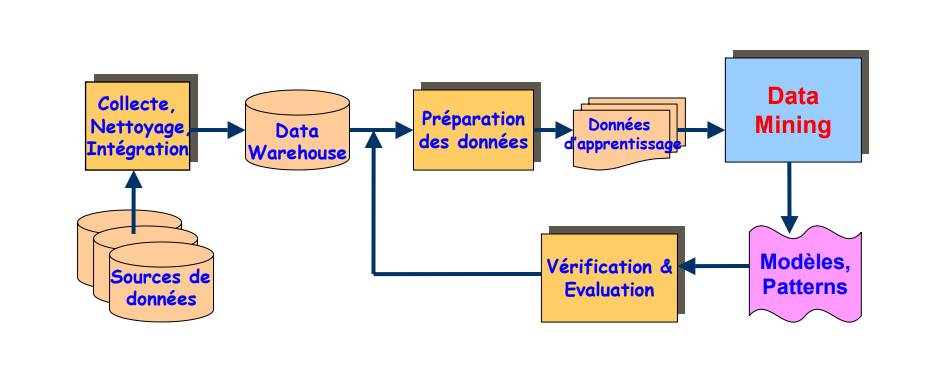
\includegraphics[width=0.75\textwidth]{KDD_data_mining}
            \caption{Data mining : coeur de KDD.}
            \label{fig:mesh1}
        \end{figure}        

        Le processus de découverte de connaissances dans les bases de données comprend plusieurs étapes, allant de la collecte de données brutes à la production de nouvelles connaissances. Ce processus itératif comprend les étapes suivantes.

        \begin{itemize}
            \item \textbf{Nettoyage des données} : il s’agit d’une phase au cours de laquelle les données parasites et les données non pertinentes sont supprimées de la collection.
            \item \textbf{Intégration des données} : à ce stade, plusieurs sources de données, souvent hétérogènes, peuvent être combinées en une source commune.
            \item \textbf{Sélection des données} : à cette étape, les données pertinentes pour l’analyse sont sélectionnées et extraites de la collecte de données.
            \item \textbf{Transformation des données} : également appelée consolidation des données, il s’agit d’une phase au cours de laquelle les données sélectionnées sont transformées sous des formes adaptées à la procédure d’exploration.
            \item \textbf{Exploration des données} : étape cruciale où des techniques astucieuses sont appliquées pour extraire des modèles potentiellement utiles.
            \item \textbf{Évaluation des modèles} : à cette étape, des modèles strictement intéressants représentant les connaissances sont identifiés sur la base de mesures données.
            \item \textbf{Représentation des connaissances} : phase finale au cours de laquelle les connaissances découvertes sont représentées visuellement à l’utilisateur. Cette étape essentielle utilise des techniques de visualisation pour aider les utilisateurs à comprendre et à interpréter les résultats de l’exploration des données. \\
        
        \end{itemize}

        Il est courant de combiner certaines de ces étapes. Par exemple, le nettoyage et l'intégration des données peuvent être réalisés conjointement lors d'une phase de prétraitement afin de générer un entrepôt de données. La sélection et la transformation des données peuvent également être combinées lorsque la consolidation des données résulte de la sélection ou, comme dans le cas des entrepôts de données, lorsque la sélection est effectuée sur des données transformées.

        Le KDD est un processus itératif. Une fois les connaissances découvertes présentées à l'utilisateur, les mesures d'évaluation peuvent être améliorées, l'exploration peut être affinée, de nouvelles données peuvent être sélectionnées ou transformées, ou de nouvelles sources de données peuvent être intégrées, afin d'obtenir des résultats différents et plus pertinents.

        Le data mining tire son nom des similitudes entre la recherche d'informations précieuses dans une grande base de données et l'extraction de minerais précieux. Ces deux techniques impliquent soit de passer au crible une grande quantité de matériaux, soit de sonder ingénieusement ces matériaux pour identifier précisément où se trouvent les valeurs. Il s'agit toutefois d'une appellation erronée, car l'extraction de l'or dans les roches est généralement appelée « extraction d'or » et non « extraction de roches ». Par analogie, l'exploration de données aurait donc dû être appelée « exploration de connaissances ». Néanmoins, l'exploration de données est devenue le terme courant et, très rapidement, une tendance qui a même éclipsé des termes plus généraux tels que la découverte de connaissances dans les bases de données (KDD), qui décrit un processus plus complet. D'autres termes similaires font référence à l'exploration de données : dragage de données, extraction de connaissances et découverte de modèles.

    \section{la méthodologie CRISP-DM}
        Développée par IBM dans les années 60, la méthodologie CRIPS-DM était conçue initialement pour des projets de Data Mining. Aujourd'hui elle est majoritairement utilisé dans les équipes de data science pour gérer les projets d’exploration et d’analyse des données.\\
        CRISP-DM, qui signifie Cross-Industry Standard Process for Data Mining, est une méthode mise à l'épreuve sur le terrain permettant d'orienter les travaux d'exploration de données.
        \begin{itemize}
            \item En tant que \textbf{méthodologie}, CRISP-DM comprend des descriptions des phases typiques d'un projet et des tâches comprises dans chaque phase, et une explication des relations entre ces tâches.
            \item En tant que \textbf{modèle de processus}, CRISP-DM offre un aperçu du cycle de vie de l'exploration de données.
        \end{itemize}
        
        \clearpage
        \begin{figure}[htbp]
                \centering
                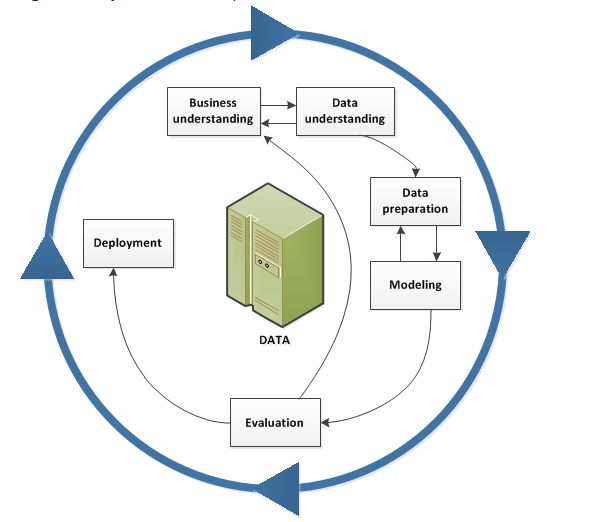
\includegraphics[width=0.75\textwidth]{crispdm}
                \caption{Le cycle de vie de l'exploration des données.}
                \label{fig:mesh1}
        \end{figure} 

        \subsection{Les étapes de CRISP-DM}
        Le modèle de cycle de vie comporte six(6) phases dotées de flèches indiquant les dépendances les plus importantes et les plus fréquentes entre les phases. La séquence des phases n'est pas strictement établie. De fait, les projets, pour la plupart, passent d'une phase à l'autre en fonction des besoins. 

            \subsubsection{Etape 1 : La compréhension du besoin client ou business understanding}
            Dans cette phase initiale, l’équipe de data science travaille en collaboration avec les parties prenantes afin de comprendre les objectifs commerciaux, les exigences, les contraintes du projet ainsi que les bénéfices attendus.\\ 
            Les ressources nécessaires pour réaliser le projet, tels que le budget, les compétences techniques et l'accès aux données, sont évalués. Les problèmes à résoudre sont identifiés et les critères permettant de mesurer le succès du projet sont définis. \\
            Cette étape est essentielle pour garantir la bonne atteinte des objectifs du projet.
    
            \subsubsection{Etape 2 : La compréhension des données ou data understanding}
            Cette phase consiste à collecter, explorer et évaluer toutes les données disponibles pour le projet. L'équipe de data science analyse ces dernières pour comprendre leur structure, leur qualité, leurs éventuels problèmes, leur pertinence et leur disponibilité. \\
            Cela permet d’identifier les valeurs manquantes, ou les erreurs qui pourraient affecter les analyses suivantes. Elle se concerte ensuite avec les experts métiers pour identifier des pistes de résolution des problèmes constatés et ainsi aider à interpréter les données.
    
            
            \subsubsection{Etape 3 : La préparation des données}
            Une fois que les données ont été évaluées, il faut à présent sélectionner les variables et les échantillons pertinents pour l’analyse, en fonction des objectifs qui ont été fixés.\\ 
            Les données sont ensuite nettoyées et, si nécessaire, transformées. Cela peut inclure la gestion des valeurs manquantes, l'échantillonnage des données et la création de variables dérivées. Si plusieurs sources de données sont utilisées, elles sont intégrées pour créer un ensemble de données cohérent.\\ 
            Cette étape monopolise plus de la moitié du temps sur l’ensemble du projet.
            
            \subsubsection{Etape 4 : La modélisation ou modeling}
            Dans cette phase, à partir de techniques d'analyse des données, l’équipe de data science construit des modèles prédictifs ou des modèles descriptifs, en fonction des objectifs du projet. Plusieurs itérations ont lieu entre les étapes de préparation et de modélisation pour affiner l’utilisation de certains algorithmes particuliers. \\
            L’étape du modeling génère souvent plusieurs modèles de Data Mining qui répondent tous à la même problématique.
    
            \subsubsection{Etape 5 : L’évaluation}
            Une fois que les modèles ont été construits, ils sont évalués pour déterminer leur qualité et leur précision. Cette étape du cycle permet de s’assurer que le modèle permet d’atteindre les objectifs du projet. \\
            Les performances des modèles sont mesurées à l'aide de métriques appropriées et comparées aux critères de succès définis dans la première phase du cycle. Si les résultats ne répondent pas aux attentes ou s'il y a des problèmes identifiés, les étapes précédentes peuvent être révisées et répétées pour améliorer les performances du modèle
    
    
            \subsubsection{Etape 6 : Le déploiement}
            Enfin, les résultats du projet sont présentés aux parties prenantes et sont intégrés si nécessaire dans les systèmes existants pour aider la prise de décision. Cette phase implique souvent la création de rapports, de visualisations ou d'autres formes de communication pour rendre les résultats compréhensibles et utilisables par ceux qui ne seraient pas spécialistes des données. \\
            A cette étape, le modèle est performant et répond correctement à la problématique.

        \subsection{Une approche agile }
        Il est important de noter que la méthodologie CRISP-DM est itérative, ce qui signifie que les différentes phases peuvent être révisées et répétées en fonction des résultats et des besoins du projet.\\
        A chaque étape d’une itération, l’équipe rédige un document qui récapitule ce qui a été fait ou ce qui a été trouvé. Ce document est mis à jour à chaque itération pour fournir ensuite un livrable complet au client.

        
\chapter{ Principales Techniques du Data Mining}

    \section{Exploration et prétraitement des données }

    \section{Types d’apprentissage}
    
        Il existe trois grandes approches en apprentissage automatique : l'apprentissage supervisé, qui utilise des données étiquetées pour prédire des résultats, l'apprentissage non supervisé, qui travaille sur des données non étiquetées pour découvrir des structures, et l'apprentissage semi-supervisé, qui combine les deux pour exploiter des données partiellement étiquetées. Chaque approche présente des nuances et excelle dans des domaines spécifiques.
        
        \subsection{Apprentissage supervisé}
        
        L'apprentissage \textbf{supervisé} repose sur des ensembles de données étiquetées, c’est-à-dire que chaque donnée d’entrée est associée à une sortie connue (comme une catégorie ou une valeur), permettant à l’algorithme d’apprendre à prédire ces sorties pour de nouvelles données. Ces ensembles de données sont conçus pour former ou « superviser » les algorithmes afin qu'ils classent les données ou prédisent les résultats avec précision. En utilisant des entrées et des sorties étiquetées, le modèle peut mesurer sa précision et apprendre au fil du temps.
        
        \subsubsection*{Objectif}
        
        \begin{itemize}
            \item  À partir des données \(\{(x_i, y_i) \in \mathcal{X} \times \mathcal{Y}, i = 1, \ldots, N\}\), où \(x_i\) représente les caractéristiques d’un exemple (comme des symptômes) et \(y_i\) son étiquette (comme un diagnostic), estimer les dépendances entre \(\mathcal{X}\) et \(\mathcal{Y}\).
            \item  On parle d'apprentissage \textbf{supervisé} car les \(y_i\) permettent de guider le processus d’estimation.
        \end{itemize}
        
        \subsubsection*{Exemples}
        
        \begin{itemize}
            \item  Prédire le risque d’infarctus à partir de données sur l’alimentation et l’âge d’un patient. Ici, \(x_i\) correspond à \(d\) attributs concernant le régime d’un patient, et \(y_i\) à sa catégorie (risque ou pas de risque).
            \item  Détecter des fraudes bancaires en analysant des transactions étiquetées comme frauduleuses ou non.
            \item  Applications : diagnostic médical, reconnaissance de caractères, prévision de la demande, etc.
        \end{itemize}
        
        \subsubsection*{Techniques}
        
        \begin{itemize}
            \item L'apprentissage supervisé peut être divisé en deux types de problèmes : la \textbf{classification} (ex. machines à vecteurs de support, arbres de décision, réseaux de neurones) et la \textbf{régression} (ex. régression linéaire, régression logistique).
        \end{itemize}
        
        \subsection{Apprentissage non supervisé}
        
        L'apprentissage \textbf{non supervisé} utilise des algorithmes pour analyser des données non étiquetées et identifier des modèles ou regroupements sans aucune indication préalable sur les résultats attendus. Ces algorithmes découvrent des structures cachées dans les données sans intervention humaine, d'où le terme « non supervisé ».
        
        \subsubsection*{Objectifs}
        
        \begin{itemize}
            \item  À partir des données \(\{x_i \in \mathcal{X}, i = 1, \ldots, N\}\), décrire l’organisation des données, extraire des sous-ensembles homogènes ou explorer des structures cachées.
        \end{itemize}
        
        \subsubsection*{Exemples}
        
        \begin{itemize}
            \item  Regrouper les clients d’un supermarché selon leurs habitudes d’achat. Ici, \(x_i\) représente un individu (adresse, âge, habitudes de courses, etc.).
            \item  Détecter des anomalies dans des données industrielles, comme des défauts de fabrication.
            \item  Applications : segmentation de marchés, catégorisation de documents, compression d’images, etc.
        \end{itemize}
        
        \subsubsection*{Techniques}
        
        \begin{itemize}
            \item Les techniques incluent le \textbf{clustering} (ex. k-means, clustering hiérarchique), l’\textbf{association} (ex. Apriori pour les règles d’association) et la \textbf{réduction de dimensionnalité} (ex. analyse en composantes principales - PCA).
        \end{itemize}
        
        \subsection{Apprentissage semi-supervisé}
        
        L'apprentissage \textbf{semi-supervisé} vise à exploiter un petit ensemble de données étiquetées \(\{(x_1, y_1), \ldots, (x_n, y_n)\}\) et un grand ensemble de données non étiquetées \(\{x_{n+1}, \ldots, x_N\}\), notamment lorsque l’étiquetage est coûteux ou chronophage. L’objectif est similaire à celui de l’apprentissage supervisé, mais en tirant parti des données non étiquetées pour améliorer la performance.
        
        \subsubsection*{Objectifs}
        
        \begin{itemize}
            \item  Utiliser les données étiquetées pour guider l’apprentissage tout en exploitant les données non étiquetées pour mieux comprendre la structure des données.
        \end{itemize}
        
        \subsubsection*{Exemples}
        
        \begin{itemize}
            \item  Classer des pages Web avec seulement quelques labels disponibles, le reste étant non étiqueté.
            \item  Améliorer la reconnaissance vocale en combinant quelques échantillons étiquetés à des données audio brutes.
            \item  Applications : traitement du langage naturel, vision par ordinateur, bioinformatique, etc.
        \end{itemize}
        
        \subsubsection*{Exemples de méthodes}
        
        \begin{itemize}
            \item Méthodes bayésiennes, machines à vecteurs de support (SVM) semi-supervisées, auto-encodeurs, etc.
        \end{itemize}
    
      \section{Tâches principales du Data Mining}
        Le data mining englobe plusieurs tâches clés visant à extraire des informations utiles et des motifs cachés à partir de grandes quantités de données. Ces tâches peuvent être réalisées à l'aide de différentes techniques d'apprentissage automatique, en fonction des objectifs et de la nature des données. Voici les principales tâches du data mining :
        
        \subsection{Classification}
        
        La \textbf{classification} est une des tâches importante du datamining. L’objectif est de construire un modèle qui permet de prédire si une instance de donnée est membre d’une classe prédéfinie.  Nous décrivons dans ce qui suit les notions de base partagées par la plupart des algorithmes utilisées dans la classification comme les arbres de décision, machines à vecteurs de support (SVM), réseaux de neurones, k-plus proches voisins (k-NN).

        \subsubsection{Principe général}


            \begin{itemize}
                \item  Objectif : apprendre un modèle à partir de données étiquetées pour prédire la classe d’objets inconnus.
                \item  Fonctionnement : le modèle est entraîné sur un ensemble de données où chaque exemple est associé à une classe, puis il est utilisé pour classer de nouvelles données.\\
            \end{itemize}
            % {\\}
            La classification utilise un ensemble $D$ de données appelées ensemble d’apprentissage. Chaque donnée est typiquement représentée sous forme d’un vecteur d’attributs 
            $x = \langle x_1, x_2, \dots, x_m, y \rangle$ avec $y$ un attribut de classe. 
            
            L’objectif de la classification est d’entraîner un algorithme de classification $A$ sur l’ensemble $S$, pour trouver une bonne approximation d’une certaine fonction $f(x) = y$. La fonction approximative $Cl$ calculée est appelée classifieur. 
            
            L’évaluation de la précision de $Cl$ est faite sur un ensemble de données $T$ indépendant de $S$, appelé ensemble de test. Le classifieur sera par la suite capable de prédire la valeur de classe $y$ pour de nouvelles données $d$, en calculant $Cl(d)$ (Figure \ref{fig:classification}).
            
            \begin{figure}[h]
                \centering
                \includegraphics[width=0.9\textwidth]{schema_classification.png}
                \caption{Schéma général de la tâche de classification}
                \label{fig:classification}
            \end{figure}
        
        \subsubsection*{Exemples}

        \begin{itemize}
            \item  Détection de spam : classer les emails comme « spam » ou « non spam ».
            \item  Diagnostic médical : prédire si un patient a une maladie spécifique en fonction de ses symptômes.
            \item  Applications : reconnaissance d’images, analyse de sentiments, prévision de churn client.
        \end{itemize}

        \subsubsection{Évaluation de la performance de la classification}

        La performance de la classification est mesurée en fonction du nombre d'instances bien classées et mal classées par le modèle. Elle est évaluée généralement par la \textit{précision} et le \textit{taux d'erreur} :
        
        \begin{itemize}
            \item \textbf{Précision (Accuracy)} = $\frac{\text{Nombre d'instances bien classées}}{\text{Nombre total d'instances}}$
            \item \textbf{Taux d'erreur (Error rate)} = $\frac{\text{Nombre d'instances mal classées}}{\text{Nombre total d'instances}}$
        \end{itemize}
        
        Ces valeurs sont mesurées sur l'ensemble de test qui peut être construit par différentes méthodes :

         \begin{itemize}
            \item  {La méthode 2/3 Apprentissage, 1/3 Test} :  L'apprentissage est réalisé sur 2/3 de l'ensemble de données, tandis que le 1/3 est réservé pour le test.
            \item  {La méthode de validation croisée}   C'est une méthode qui consiste à diviser l'ensemble $D$ en $k$ parties disjointes $\{D_1, D_2, ... D_k\}$. Le processus suivant est répété $k$ fois (Figure 2.6) : construction d'un classificateur $Cl_i$ avec l'ensemble privé de $D_i$ ($D - D_i$), ensuite évaluation de la précision de $Cl_i$ en utilisant les données $D_i$. La précision globale est obtenue par la moyenne. Les ensembles construits de cette manière sont appelés \textit{cross validated committees}.
        \end{itemize}
  
        \subsubsection*{Techniques}

        \subsubsection*{a) Arbres de Décision}

            Un arbre de décision est un modèle prédictif sous forme d'une structure arborescente, où chaque nœud interne représente une "question" ou un "test" sur une caractéristique (par exemple, si une valeur numérique est supérieure à un seuil donné ou si une catégorie spécifique est présente). Chaque branche descendante de ce nœud correspond à l'une des réponses possibles à cette question, et chaque nœud feuille (ou terminal) de l'arbre représente une prédiction ou une décision prise à la suite des réponses aux questions précédentes. 
             \subsubsection{Fonctionnement :}
            - Construction de l'arbre : À partir d'un ensemble de données d'entraînement, l'algorithme divise l'ensemble en sous-ensembles en utilisant une méthode de sélection de caractéristiques basée sur des critères comme l'indice de Gini, l'entropie ou la réduction de la variance. Ce processus est répété de manière récursive jusqu'à ce qu'un critère d'arrêt soit atteint, comme une profondeur maximale de l'arbre ou un nombre minimal d'échantillons dans un nœud feuille.
            
            - Prédiction : Pour faire une prédiction, on suit le chemin dans l'arbre en partant de la racine, en posant les questions correspondant à chaque nœud interne en fonction des caractéristiques de l'instance à classer ou à évaluer, jusqu'à atteindre un nœud feuille qui donne la prédiction finale.
            
            \subsubsection{ Exemples d'application :}

            \begin{itemize}
                \item Diagnostic médical : Un arbre de décision peut être utilisé pour diagnostiquer des maladies en se basant sur les symptômes et les résultats d'examens des patients. Chaque nœud interne représenterait un symptôme ou un résultat de test, et les nœuds feuilles représenteraient les diagnostics possibles

                 \begin{figure}[h]
                    \centering
                    \includegraphics[width=0.9\textwidth]{images/decision tree example.png}
                    \caption{decision tree example}
                    \label{fig:decision tree example}
                \end{figure}
                \item Sélection de candidat : Les entreprises peuvent utiliser les arbres de décision pour filtrer les candidats à un poste en fonction de différents critères comme l'expérience, les compétences, l'éducation et les performances aux tests d'évaluation. L'arbre pourrait aider à décider si un candidat doit passer à l'étape suivante du processus de recrutement.
            \end{itemize}
            
        \subsubsection*{b) Machines à Vecteurs de Support (SVM)}
        La machine à vecteurs de support (SVM, pour "Support Vector Machine" en anglais) est une méthode d'apprentissage supervisé utilisée pour la classification et la régression. Elle vise à trouver l'hyperplan optimal qui sépare au mieux les différentes classes de données dans l'espace des caractéristiques. Cet hyperplan est choisi de manière à maximiser la marge entre les deux classes les plus proches de l'hyperplan, ces données étant appelées vecteurs de support.
        
        Les SVM sont particulièrement efficaces dans les espaces de grande dimension et dans les cas où le nombre de dimensions dépasse le nombre d'échantillons. Ils sont également polyvalents grâce à l'utilisation de fonctions noyau (kernel functions), qui permettent de traiter les données linéairement non séparables en les projetant dans un espace de plus grande dimension où elles deviennent séparables.
        
        \subsubsection{Exemples d'application :}
        
        Reconnaissance de visages : Les SVM peuvent être utilisés pour identifier les personnes à partir de caractéristiques extraites de leurs visages, ce qui est utile dans les systèmes de sécurité et de surveillance.
        
        \subsubsection*{c) Réseaux de Neurones}
        Les réseaux de neurones sont des modèles d’apprentissage automatique inspirés du cerveau humain, composés de couches de neurones interconnectés pour traiter des données et apprendre des patterns complexes.
        Ils sont constitués de couches de neurones interconnectés : une couche d’entrée, une ou plusieurs couches cachées, et une couche de sortie. Chaque neurone calcule une combinaison linéaire de ses entrées (pondérées par des poids) et applique une fonction d’activation pour produire une sortie.

        L’apprentissage consiste à ajuster les poids pour minimiser une fonction de perte, qui mesure l’écart entre les prédictions du réseau et les vraies étiquettes. Cet ajustement se fait via la rétropropagation du gradient, qui propage l’erreur de la sortie vers l’entrée pour mettre à jour les poids.

        \subsubsection{Applications de la classification par réseaux de neurones en data mining:}

        1. Reconnaissance d'images: Les réseaux de neurones convolutifs (CNN) sont largement utilisés pour classer des images dans des catégories, telles que la reconnaissance faciale ou l'identification d'objets.
        
        2. Diagnostic médical: Les réseaux de neurones peuvent être entraînés pour classer des images médicales (comme des radiographies ou des IRM) pour aider à identifier des conditions ou des maladies spécifiques.
        
        3. Détection de fraude: Dans le secteur financier, les réseaux de neurones peuvent être utilisés pour classer les transactions en tant que légitimes ou frauduleuses, en se basant sur des motifs complexes dans les données.

        
%         \subsubsection*{d) k-Plus Proches Voisins (k-NN)}
%         k-NN est un algorithme paresseux, c’est-à-dire qu’il ne construit pas de modèle explicite pendant l’entraînement. Pour classer une nouvelle donnée, il identifie les k échantillons les plus proches dans l’ensemble d’entraînement et attribue la classe majoritaire parmi ces voisins.

% La proximité est généralement mesurée avec la distance euclidienne(\( \sqrt{\sum (x_i - y_i)^2} \)), mais d’autres métriques comme la distance de Manhattan peuvent être utilisées selon le contexte.

        \subsection{Clustering ( Segmentation )}
        
        Le \textbf{clustering} (ou regroupement) vise à regrouper des objets similaires en clusters, sans utiliser de classes prédéfinies. Il est utilisé pour découvrir des structures ou des motifs cachés dans des données non étiquetées.
        
        \subsubsection*{Principe général}
        
        \begin{itemize}
            \item  Objectif : identifier des groupes naturels dans les données, où les objets d’un même cluster sont plus similaires entre eux que ceux des autres clusters.
            \item  Fonctionnement : les algorithmes de clustering analysent les similitudes entre les objets et les regroupent en conséquence.\\
        \end{itemize}
        % {\\}
        Formellement : Soit X un ensemble de N données décrites chacune par leurs P
        attributs, la segmentation consiste a créer une décomposition de cet ensemble
        en groupes telle que les données appartenant au même groupe se ressemblent,
        tandis que les données appartenant a deux groupes différents soient peu
        ressemblantes.{\\}{\\}
        Le problème de segmentation optimale en k groupes est NP-complet. Il faut
        donc chercher des algorithmes calculant une bonne décomposition, sans
        espérer être sûr de trouver la meilleure. On distingue essentiellement deux 
        types de méthodes «non hiérarchiques» ou «hiérarchques».
        L’outils de base dans cette tâche est la mesure de similarité entre les données.
        
        \subsubsection*{Mesures de similarité}

        La méthode de calcul de distance entre deux objets dépend essentiellement de
        la nature des données à segmenter (Euclidienne, Jaccard, Hamming,
        Menhatten, ...). La figure (Figure \ref{fig:distance_eulidienne}) présente un exemple de calcul de la distance
        euclidienne entre deux objets.
            
        \begin{figure}[h]
            \centering
            \includegraphics[width=0.9\textwidth]{schema_distance_eulidienne.png}
            \caption{Exemple de calcul de la distance euclidienne}
            \label{fig:distance_eulidienne}
        \end{figure}

        \subsubsection*{Approche non hiérarchique}

        L'ensemble d'objets est décomposé en groupes. L’algorithme le plus répandu
        dans cette approche est «k-means» . La méthode du choix de la
        valeur de k (nombre de centroides initial) est un champs d’investigation. Par
        défaut, k est choisi aléatoirement. Le critère d’arrêt peut être soit la stabilisation
        des objets, ou bien d’autre mesures comme l’inertie. \\


        \begin{enumerate}[leftmargin=*]
            \item Déterminer le nombre de Clusters \( K\)
            \item Prendre \( K \) objets arbitraires «~centroides~»
            \item Calculer les distances entre les objets et les centroides
            \item Grouper les objets selon la distance minimale
            \item Si aucun objet ne change de groupes, alors fin
            \item Sinon calculer les nouveaux centroides, aller à 4
        \end{enumerate}
        
        Principe général de l’algorithme \( k \)-means

        \subsubsection*{Approche hiérarchique}
        On décompose l'ensemble d'objets en une arborescence de groupes
        (dendogramme). Le principe consiste à débuter de N groupes, que l'on réduit à
        N-1, puis a N-2.... etc. On passe donc de k+1 a k groupes en regroupant deux
        groupes. 
        \\
        \begin{enumerate}[leftmargin=*]
            \item Calculer la matrice des distances
            \item Chaque objet représente un Cluster
            \item Regrouper les deux clusters les plus proches
            \item Mettre à jour la matrice des distances
            \item Si le nombre de Clusters = 1, fin Sinon, aller à 3
          \end{enumerate}
        
        Principe de base du clustering hiérarchique
        
        \subsubsection*{Exemples}

        
        \begin{itemize}
            \item  Segmentation de marché : regrouper les clients en fonction de leurs comportements d’achat.
            \item  Analyse de données sociales : identifier des communautés dans les réseaux sociaux.
            \item  Applications : compression d’images, recommandation de contenu, biologie (classification de gènes).
        \end{itemize}
        
        % \subsubsection*{Techniques}
        
        % \begin{itemize}
        %     \item K-means, DBSCAN, clustering hiérarchique, Gaussian Mixture Models (GMM).
        % \end{itemize}
      
      \subsection{Régression}

La \textbf{régression} est une tâche du data mining qui vise à prédire une valeur numérique continue en fonction d'une ou plusieurs variables prédictives. Contrairement à la classification, qui prédit des étiquettes de classe catégoriques, la régression modélise des fonctions à valeurs continues. Elle est particulièrement utile lorsque les variables prédictives sont également continues.

\subsubsection*{Principe général}

\begin{itemize}
    \item  Objectif : apprendre un modèle à partir de données étiquetées pour prédire une valeur numérique pour de nouvelles données.
    \item  Fonctionnement : le modèle est entraîné sur un ensemble de données où chaque exemple est associé à une valeur cible continue, puis il est utilisé pour prédire cette valeur pour de nouvelles instances.
\end{itemize}

La régression cherche à modéliser la relation entre une variable dépendante \( y \) (la variable à prédire) et une ou plusieurs variables indépendantes \( x_1, x_2, \dots, x_n \) (les prédicteurs). Le modèle de régression le plus simple est la régression linéaire, où la relation est supposée linéaire.

\subsubsection*{Techniques}

Les techniques de régression incluent :

\begin{itemize}
    \item \textbf{Régression linéaire} : modélise la relation entre les variables par une ligne droite. Pour un seul prédicteur, elle prend la forme \( y = w_0 + w_1 x \), où \( w_0 \) et \( w_1 \) sont les coefficients à estimer. Ces coefficients sont souvent estimés par la méthode des moindres carrés, qui minimise la somme des carrés des erreurs entre les valeurs observées et prédites. Les formules sont :
    \[
    w_1 = \frac{\sum_{i=1}^D (x_i - \bar{x})(y_i - \bar{y})}{\sum_{i=1}^D (x_i - \bar{x})^2}, \quad w_0 = \bar{y} - w_1 \bar{x}
    \]
    où \( \bar{x} \) et \( \bar{y} \) sont les moyennes des \( x_i \) et \( y_i \), respectivement.


    Exemple : Prédiction du salaire : estimer le salaire d’un employé en fonction de son expérience professionnelle.

    \begin{figure}[h!]
        \begin{minipage}[b]{0.5\textwidth}
            \centering
            \includegraphics[width=\textwidth]{images/linear_data.png} 
            \caption{Table Data}
        \end{minipage}%
        \begin{minipage}[b]{0.5\textwidth}
            \centering
            \includegraphics[width=\textwidth]{images/linear_representation.png} 
            \caption{2-D data on a scatter plot.}
        \end{minipage}
    \end{figure}

        % Début de la mise en page en deux colonnes
        \begin{minipage}[t]{0.48\textwidth} % Colonne de gauche (texte)
        \vspace{0pt} % Alignement vertical
        
        À partir des données ci-dessus, nous calculons :
        \[
        \bar{x} = 9{,}1 \quad \text{et} \quad \bar{y} = 55{,}4
        \]
        
        Nous obtenons :
        \[
        w_1 = \frac{(3 - 9{,}1)(30 - 55{,}4) + \cdots + (16 - 9{,}1)(83 - 55{,}4)}{(3 - 9{,}1)^2 + \cdots + (16 - 9{,}1)^2} = 3{,}5
        \]
        
        \[
        w_0 = 55{,}4 - (3{,}5)(9{,}1) = 23{,}6
        \]
        
        L'équation de la droite des moindres carrés :
        \[
        y = 23{,}6 + 3{,}5x
        \]
        
        \end{minipage}
        
    
       \begin{figure}[h]
            \centering
            \includegraphics[width=0.9\textwidth]{images/linear_regression.png}
            \caption{Exemple de régression linéaire}
            \label{fig:reg}
        \end{figure}

    \item \textbf{Régression linéaire multiple} :  La régression linéaire multiple implique l'utilisation de plusieurs variables prédictives.   Les données d'apprentissage sont de la forme :
    \[
    (\mathbf{X}_1, y_1),\ (\mathbf{X}_2, y_2),\ \dots,\ (\mathbf{X}_p, y_p)
    \]
    où :
    \begin{itemize}
        \item $\mathbf{X}_i \in \mathbb{R}^n$ : vecteur de données de dimension $n$
        \item $y_i$ : étiquette de classe associée
    \end{itemize}
    
    c'extension de la régression linéaire à plusieurs prédicteurs, de la forme \( y = w_0 + w_1 x_1 + w_2 x_2 + \dots + w_n x_n \). Elle permet de modéliser des relations plus complexes en tenant compte de plusieurs variables.

    \item \textbf{Régression non linéaire} : utilisée lorsque la relation entre les variables n’est pas linéaire. Par exemple, la régression polynomiale : \( y = w_0 + w_1 x + w_2 x^2 + w_3 x^3 \). Elle peut capturer des relations plus complexes mais nécessite plus de données et peut être sujette au surajustement.
  
    \item \textbf{Modèles linéaires généralisés} : incluent la régression logistique, qui modélise la probabilité d’un événement, et la régression de Poisson, pour des données de comptage. Ils étendent la régression linéaire à des distributions non normales.

    \item \textbf{Arbres de régression et arbres de modèle} : des arbres de décision où les feuilles prédisent des valeurs numériques. Les arbres de régression prédisent la moyenne des instances atteignant la feuille, tandis que les arbres de modèle utilisent des modèles de régression dans les feuilles. Ils sont utiles pour des données non linéaires et peuvent être plus précis que les modèles linéaires simples.
\end{itemize}

\subsubsection*{Évaluation de la performance}

La performance des modèles de régression est évaluée à l’aide de métriques telles que :

\begin{itemize}
    \item \textbf{Erreur quadratique moyenne (MSE)} : \(\frac{1}{n} \sum_{i=1}^n (y_i - \hat{y}_i)^2\)
    \item \textbf{Erreur absolue moyenne (MAE)} : \(\frac{1}{n} \sum_{i=1}^n |y_i - \hat{y}_i|\)
    \item \textbf{Coefficient de détermination (R²)} : \(1 - \frac{\sum_{i=1}^n (y_i - \hat{y}_i)^2}{\sum_{i=1}^n (y_i - \bar{y})^2}\)
\end{itemize}

Ces métriques sont calculées sur un ensemble de test indépendant pour évaluer la capacité du modèle à généraliser à de nouvelles données.

Il est également important de sélectionner les attributs pertinents pour éviter le surajustement et d’identifier les valeurs aberrantes qui peuvent fausser les résultats de la régression.

En conclusion, la régression est une technique puissante pour la prédiction numérique, offrant une gamme de modèles adaptés à différents types de données et de relations entre variables.  
        \subsection{Détection d’anomalies}

        \subsection{Extraction de règles d’association}
        
        L'\textbf{extraction de règles d’association} est une tâche fondamentale en fouille de données (data mining), visant à identifier des relations implicites et significatives entre les attributs dans de grandes bases de données. Introduite par Agrawal et al. , cette technique est particulièrement reconnue pour son application dans l’analyse du panier de marché. Elle permet, par exemple, de dégager des règles telles que « 70\% des clients achetant du lait et du thé achètent aussi du pain », utiles pour optimiser l’agencement des rayons, planifier des promotions ou gérer les stocks dans un objectif d’amélioration des profits.
        
        Dans ce contexte, une base de données transactionnelle est un ensemble de transactions, où chaque transaction représente un sous-ensemble d’attributs (ou items) achetés par un client. Une règle d’association est une implication conditionnelle de la forme \( X \rightarrow Y \), où \( X \) et \( Y \) sont des ensembles d’attributs disjoints, exprimant que l’occurrence de \( X \) dans une transaction est souvent associée à celle de \( Y \). Le problème est complexe en raison du nombre exponentiel d’attributs possibles et du volume des bases transactionnelles, qui peuvent contenir des millions de transactions sur des milliers d’attributs.
        
        % Ce chapitre explore les processus d’extraction des règles d’association dans un contexte binaire. Il est structuré comme suit : la problématique est exposée dans la Section \ref{sec:prob_assoc}, les définitions et principes de base, incluant l’algorithme APRIORI, sont présentés dans la Section \ref{sec:def_principes}, les représentations condensées des motifs fréquents sont abordées dans la Section \ref{sec:rep_condensees}, et une conclusion est donnée dans la Section \ref{sec:concl_assoc}.
        
        \subsubsection{Problématique}
        \label{sec:prob_assoc}
        
        Le cadre classique de la fouille des règles d’association peut être décrit ainsi : soit \( A = \{x_1, x_2, \dots, x_m\} \) un ensemble de \( m \) attributs (ou items), et \( E = \{e_1, e_2, \dots, e_n\} \) un ensemble de \( n \) transactions, chaque transaction \( e_i \) étant un sous-ensemble de \( A \). Chaque transaction est associée à un identifiant unique (TID, Transaction IDentifier). Un motif est un sous-ensemble de \( A \), et une règle d’association est une implication \( X \rightarrow Y \) (où \( Y \neq \emptyset \)), indiquant que les attributs de \( X \) tendent à apparaître avec ceux de \( Y \).
        
        Les mesures clés pour évaluer une règle sont :
        \begin{itemize}
            \item Le \textbf{support} d’un motif \( X \), défini par \( \text{Supp}(X) = \frac{|\{e \in E \mid X \subseteq e\}|}{|E|} \), soit la proportion de transactions contenant \( X \).
            \item Le \textbf{support} d’une règle \( X \rightarrow Y \), égal à \( \text{Supp}(X \cup Y) \).
            \item La \textbf{confiance} d’une règle, définie par \( \text{Conf}(X \rightarrow Y) = \frac{\text{Supp}(X \cup Y)}{\text{Supp}(X)} \), soit la proportion de transactions contenant \( Y \) parmi celles contenant \( X \).
        \end{itemize}
        
        Le problème consiste à identifier toutes les règles valides, c’est-à-dire celles dont le support et la confiance dépassent des seuils minimaux prédéfinis, \( \text{minsupp} \) et \( \text{minconf} \). Ce problème est décomposé en deux étapes \cite{HGN00} :
        \begin{enumerate}
            \item Trouver tous les \textbf{motifs fréquents}, i.e., les motifs dont \( \text{Supp}(X) \geq \text{minsupp} \).
            \item Générer les règles d’association valides à partir de ces motifs fréquents.
        \end{enumerate}
        
        La première étape est la plus coûteuse, car l’espace de recherche des motifs fréquents est exponentiel. Dans les bases fortement corrélées ou avec un \( \text{minsupp} \) faible, le nombre de motifs peut devenir ingérable, nécessitant des optimisations comme les représentations condensées.
        
        \subsubsection{Définitions et principes de base}
        \label{sec:def_principes}
        
        Soit \( K = (E, A, R) \) un contexte de fouille de données, où \( R \) est une relation binaire entre les transactions \( E \) et les attributs \( A \). Les définitions fondamentales sont les suivantes :
        \begin{itemize}
            \item Un \textbf{motif} \( X \subseteq A \) est un ensemble d’attributs.
            \item Un motif est \textbf{fréquent} si \( \text{Supp}(X) \geq \text{minsupp} \).
            \item Une \textbf{règle d’association} \( X \rightarrow Y \) est valide si \( \text{Supp}(X \cup Y) \geq \text{minsupp} \) et \( \text{Conf}(X \rightarrow Y) \geq \text{minconf} \).
        \end{itemize}
        
        \paragraph{L’algorithme APRIORI}
        
        L’algorithme \textbf{APRIORI} \cite{AS94} est une méthode pionnière pour extraire les motifs fréquents. Il repose sur la propriété d’anti-monotonicité du support : si un motif \( X \) est fréquent, tous ses sous-ensembles le sont aussi ; inversement, si \( X \) n’est pas fréquent, aucun de ses sur-ensembles ne l’est. Formellement :
        \begin{itemize}
            \item Si \( X \subseteq Y \), alors \( \text{Supp}(X) \geq \text{Supp}(Y) \).
            \item Si \( X \) est fréquent, tout \( X_1 \subseteq X \) l’est aussi.
            \item Si \( X \) n’est pas fréquent, tout \( X_2 \supseteq X \) ne l’est pas.
        \end{itemize}
        
        L’algorithme procède itérativement :
        \begin{enumerate}
            \item Initialisation : trouver les 1-motifs fréquents (\( F_1 \)).
            \item Pour chaque niveau \( k \geq 2 \) :
                \begin{enumerate}
                    \item Générer les candidats \( C_k \) à partir des motifs fréquents \( F_{k-1} \) (via une jointure et un élagage basé sur l’anti-monotonicité).
                    \item Calculer le support des candidats en parcourant la base.
                    \item Retenir les motifs fréquents \( F_k = \{c \in C_k \mid \text{Supp}(c) \geq \text{minsupp}\} \).
                \end{enumerate}
            \item Arrêt : lorsque \( F_{k-1} = \emptyset \).
        \end{enumerate}
        
        Le pseudo-code est le suivant :
        \begin{verbatim}
        Entrée : K (base transactionnelle), minsupp
        Sortie : F (ensemble des motifs fréquents)
        1: F_1 ← {1-motifs fréquents}
        2: for (k ← 2; F_{k-1} ≠ ∅; k++)
        3:     C_k ← Apriori-Gen(F_{k-1})
        4:     for all e ∈ E
        5:         C_E ← {c ∈ C_k | c ⊆ e}
        6:         for all c ∈ C_E
        7:             Supp(c)++
        8:         end for
        9:     F_k ← {c ∈ C_k | Supp(c) ≥ minsupp}
        10: end for
        11: Retourner F ← ∪_k F_k
        \end{verbatim}
        
        \paragraph{Génération des règles}
        
        À partir des motifs fréquents \( F \), pour chaque motif \( I \in F \), on génère les règles \( X \rightarrow Y \) (où \( I = X \cup Y \), \( Y \neq \emptyset \)) en vérifiant \( \text{Conf}(X \rightarrow Y) \geq \text{minconf} \). Une optimisation \cite{AS94} exploite la propriété suivante : si \( I_1 \rightarrow I \setminus I_1 \) est valide, alors toute règle avec une prémisse \( I_2 \subset I_1 \) l’est aussi, réduisant ainsi le nombre de règles à tester.
        
        \subsubsection{Représentations condensées}
        \label{sec:rep_condensees}
        
        L’extraction exhaustive des motifs fréquents peut être prohibitive en termes de temps et de mémoire. Les \textbf{représentations condensées} sont des sous-ensembles compacts de motifs fréquents permettant de dériver l’ensemble complet des motifs et leurs supports. Voici quelques approches :
        
        \paragraph{Motifs fermés fréquents}
        
        Un motif \( X \) est \textbf{fermé} si aucun sur-ensemble n’a le même support (\( \phi(X) = X \), où \( \phi \) est un opérateur de fermeture). L’ensemble des motifs fermés fréquents \( FF = \{X \subseteq A \mid \phi(X) = X, \text{Supp}(X) \geq \text{minsupp}\} \) est une représentation condensée \cite{PBTL99a}. L’algorithme CLOSE génère ces motifs efficacement.
        
        \paragraph{Motifs libres}
        
        Un motif \( X \) est \textbf{\( \delta \)-libre} s’il n’existe pas de règle \( X_1 \rightarrow X_2 \) basée sur \( X = X_1 \cup X_2 \) avec peu d’exceptions (\( \text{Supp}(X_1) - \text{Supp}(X_1 \cup X_2) \leq \delta \)) \cite{BB00}. L’ensemble \( \text{FreqFree}(E, \sigma, \delta) \) des motifs \( \delta \)-libres fréquents, combiné à sa bordure négative, offre une représentation \( \epsilon \)-adéquate \cite{BBR03}.
        
        \paragraph{Motifs essentiels}
        
        Un motif \( X \) est \textbf{essentiel} si son support disjonctif \( \text{Supp}(\vee X) \) diffère de celui de ses sous-ensembles directs \cite{CCL05}. L’union des motifs essentiels fréquents et de la bordure positive \( \text{Bd}^+(F) \) forme une couverture parfaite des motifs fréquents.
        
        \paragraph{Motifs non dérivables}
        
        Un motif \( I \) est \textbf{non dérivable} si son support ne peut être exactement déduit des supports de ses sous-ensembles via des règles d’inclusion-exclusion \cite{CG06}. L’ensemble \( \text{NDIRep} \) des motifs non dérivables fréquents est une représentation condensée.
        
        % \subsubsection{Conclusion}
        % \label{sec:concl_assoc}
        
        % L’extraction des règles d’association est essentielle pour révéler des relations cachées dans les données. La recherche des motifs fréquents, bien que coûteuse, est optimisée par les représentations condensées (motifs fermés, libres, essentiels, non dérivables), qui réduisent le nombre de motifs à traiter tout en conservant l’information nécessaire. Cependant, le grand nombre de règles générées reste un défi, menant à des approches comme les bases de règles, sous-ensembles minimaux permettant de dériver toutes les règles valides, sujet exploré dans d’autres travaux.

        


\chapter{Outils et Langages utilisés}
Il existe une multitude d’outils pour effectuer des tâches de Data Mining. Voici quelques-uns des outils les plus populaires, chacun offrant ses propres fonctionnalités et avantages :

    \section{Le language R}
    \textbf{R} est un \emph{langage de programmation} statistique avec de nombreuses bibliothèques pour la fouille de données.  Un des atouts de R est la facilité avec laquelle des graphiques bien conçus, de qualité digne de publication, peuvent être produits, contenant des symboles mathématiques et des formules si besoin est. Un grand soin a été accordé à la prise en charge des options par défaut pour les choix mineurs dans la conception des graphiques, mais l'utilisateur conserve le contrôle complet de ces options. R est publié selon les termes de la licence GNU sous forme de code source. Il se compile et s'exécute sous une grande variété de plates-formes UNIX et de systèmes similaires, y compris FreeBSD et Linux, Windows et MacOS.
    
    \section{Python}
    \textbf{Python} est un \emph{langage de programmation} polyvalent largement utilisé dans le domaine de la Data Science et du Data Mining. Il offre une vaste gamme de bibliothèques et de frameworks tels que Pandas, NumPy, scikit-learn, TensorFlow, etc., qui permettent d’effectuer diverses tâches d’analyse de données, de modélisation et de visualisation.

    \section{RapidMiner}
    \textbf{RapidMiner} est une plateforme de Data Science qui propose une interface conviviale pour la préparation des données, la modélisation, l’évaluation et le déploiement des modèles. Il offre une grande variété d’algorithmes de Data Mining et de fonctionnalités de traitement des données, ce qui en fait un choix populaire parmi les professionnels du domaine.

    
    \section{WEKA}
    \textbf{WEKA} (Waikato Environment for Knowledge Analysis) est un logiciel open source développé par l'Université de Waikato. L'outil de data mining est basé sur Java et peut être utilisé avec Windows, MacOS et Linux. Reconnu pour ses capacités étendues d'apprentissage machine, il prend en charge toutes les principales tâches d'exploration de données telles que la mise en grappe, l'association, la régression ou la classification. L'interface utilisateur graphique facilite l'accès au logiciel. En outre, WEKA offre la connexion aux bases de données SQL et peut traiter les données demandées. La force de WEKA réside dans la classification : l'outil de data mining est connu pour ses nombreuses classifications, y compris les réseaux neuronaux artificiels, les arbres de décision, les algorithmes ID3 ou C4.5. Cependant, WEKA est moins puissant dans d'autres techniques telles que l'analyse cluster. Seules les procédures les plus importantes sont proposées ici. Un autre inconvénient : WEKA peut rencontrer des problèmes de traitement si de grandes quantités de données doivent être manipulées ; en effet, l'outil d'exploration de données essaye de les charger toutes dans la mémoire de travail. Pour s'en sortir, WEKA propose une ligne de commande simple qui facilite le traitement de grandes quantités de données. 

    
    \section{Orange}
    \textbf{Orange} est une suite logicielle open-source qui offre des outils de visualisation de données, de modélisation prédictive et de Data Mining. Il propose une interface graphique intuitive qui permet aux utilisateurs de créer et d’exécuter des workflows de traitement de données sans écrire de code, ce qui le rend accessible aux débutants et aux experts.

    
    \section{KNIME}
    \textbf{KNIME} est une plateforme open-source qui permet aux utilisateurs de créer des workflows visuels pour l’analyse des données et le déploiement de modèles. Il propose une large gamme de modules pour le Data Mining, la manipulation de données, la visualisation et plus encore. KNIME est apprécié pour sa flexibilité et sa capacité à intégrer des outils et des technologies externes.
    
    \section{SAS}
    \textbf{SAS Enterprise Miner} est une solution logicielle robuste conçue pour l’analyse prédictive et le Data Mining. Il offre une large gamme d’algorithmes de modélisation avancés, une interface conviviale pour la création de workflows et des fonctionnalités de déploiement de modèles. SAS Enterprise Miner est largement utilisé dans les entreprises pour résoudre des problèmes complexes liés à l’analyse de données.



\chapter{Défis et limites du data mining}
	Nous avons vu que le data mining consiste en l’exploration d’une grande quantité de données. De ce fait, on se demande quelles machines peuvent permettre de faire du data mining. De plus, les données de mauvaise qualité peuvent mener à des analyses erronées, des décisions mal informées et, in fine, à des pertes financières et réputationnelles significatives. Cela nous pousse à nous poser des questions sur l’aspect éthique du data mining. 

	\section{Qualité et biais des données}
	    \textbf{Les biais} dans le data mining représentent des distorsions systématiques qui peuvent fausser les analyses et conduire à des décisions inappropriées. Ces biais peuvent émerger à différentes étapes du processus d'analyse de données, depuis la collecte jusqu'à l'interprétation des résultats.

		\subsection{Types de Biais Courants dans le Data Mining}
			\begin{itemize}
				\item \textbf{Biais de sélection :} Ce biais survient lorsque l'échantillon de données analysé n'est pas représentatif de la population cible. Par exemple, si une enquête est menée uniquement auprès d'une tranche d'âge spécifique, les conclusions ne seront pas généralisables à l'ensemble de la population.​
				\item \textbf{Biais de Confirmation :} Il s'agit de la tendance à privilégier les données qui confirment des hypothèses préexistantes, tout en négligeant celles qui les contredisent. Cela peut conduire à une interprétation partiale des résultats et à des conclusions erronées.​
				\item \textbf{Biais de Survivance :} Ce biais apparaît lorsque l'analyse ne prend en compte que les sujets ou entités ayant "survécu" à un certain processus, ignorant ceux qui ont échoué ou disparu. Par exemple, étudier uniquement les entreprises prospères pour déterminer les facteurs de succès sans considérer celles qui ont échoué peut mener à des conclusions biaisées.​
				\item \textbf{Biais de Mesure :} Ce biais est introduit par des erreurs dans la collecte ou la mesure des données, telles que des instruments défectueux ou des méthodes de collecte inconsistantes, affectant la précision des analyses.​
			\end{itemize}
			
		\subsection{Conséquences des Biais dans le Data Mining}
			Les biais peuvent entraîner des modèles prédictifs imprécis, des décisions commerciales inappropriées et, dans certains cas, des discriminations envers certains groupes. Par exemple, un algorithme de recrutement biaisé peut favoriser indûment un groupe démographique au détriment d'un autre, perpétuant ainsi des inégalités.


		\subsection{Stratégies pour Surmonter ces Défis}
			\begin{itemize}
				\item \textbf{Évaluation et nettoyage des données :} Mettre en place des processus rigoureux de validation et de nettoyage des données pour identifier et corriger les erreurs, éliminer les doublons et traiter les valeurs manquantes. 
				\item \textbf{Standardisation et normalisation :} Uniformiser les formats et les structures de données pour assurer la cohérence et faciliter l'intégration de sources diverses. 
				\item \textbf{Détection et Correction des Biais :} Analyser les données pour détecter les biais potentiels, en évaluant la représentativité des échantillons et en ajustant les modèles pour atténuer les effets des biais identifiés. 
				\item \textbf{Gouvernance des Données :} Établir des politiques claires de gestion des données, définir des responsabilités et mettre en place des contrôles pour maintenir la qualité et l'intégrité des données. 
				\item \textbf{Formation et Sensibilisation :} Former les équipes aux bonnes pratiques de gestion des données et les sensibiliser aux impacts des biais pour encourager une culture de qualité des données au sein de l'organisation.
			\end{itemize}

	\section{Complexité et coûts de calcul}
		Les ensembles de données modernes sont souvent caractérisés par leur volume massif, leur variété de formats et leur vitesse de génération, ce qui accroît la complexité de leur gestion et de leur analyse. Les données peuvent être stockées dans divers formats tels que des fichiers texte, des bases de données relationnelles ou des entrepôts de données, rendant leur intégration et leur préparation pour l'analyse particulièrement ardues. De plus, la diversité des sources de données nécessite des techniques avancées pour assurer une cohérence et une qualité optimales des informations exploitées.

		L'analyse de ces vastes ensembles de données requiert des ressources computationnelles considérables. Les algorithmes de data mining, en particulier ceux traitant des données massives, peuvent être très gourmands en temps et en puissance de calcul. Cette exigence se traduit par des investissements substantiels dans des infrastructures matérielles performantes, des solutions de stockage adaptées et des logiciels spécialisés. Par ailleurs, la gestion et la maintenance de ces systèmes engendrent des coûts opérationnels non négligeables.


	\section{Protection de la vie privée et éthique}
		Nous savons que le data mining consiste à extraire des informations significatives à partir de vastes ensembles de données. Cependant, cette pratique soulève des défis majeurs en matière de protection de la vie privée et d'éthique.

		\subsection{Protection de la Vie Privée}
		L'exploitation massive des données peut entraîner des atteintes à la vie privée si des informations personnelles sont utilisées sans consentement ou de manière inappropriée. Les défis incluent :
			\begin{itemize}
				\item \textbf{Collecte et Stockage des Données Personnelles :} La collecte excessive de données sensibles sans mesures de sécurité adéquates peut exposer ces informations à des violations.
				\item \textbf{Partage et Vente de Données :} Les entreprises peuvent partager ou vendre des données personnelles sans que les individus concernés en soient informés, compromettant leur confidentialité.
				\item \textbf{Profilage et Surveillance :} L'analyse des comportements individuels peut conduire à une surveillance intrusive, limitant les libertés personnelles.
			\end{itemize}

		\subsection{Considérations Éthiques}
		Au-delà de la vie privée, le data mining pose des questions éthiques :
			\begin{itemize}
				\item \textbf{Biais Algorithmiques :} Les algorithmes peuvent reproduire ou amplifier des biais existants, entraînant des discriminations.
				\item \textbf{Transparence et Consentement :} L'absence de transparence sur l'utilisation des données et le manque de consentement éclairé des individus posent des problèmes éthiques.
				\item \textbf{Utilisation Abusive des Données :} Les informations obtenues peuvent être exploitées à des fins nuisibles, comme la manipulation ou la discrimination.
			\end{itemize}
			
		\subsection{Mesures pour Atténuer ces Défis}
			\begin{itemize}
				\item \textbf{Renforcement des Régulations :} Adopter et appliquer des lois strictes sur la protection des données pour encadrer leur collecte et utilisation.
				\item \textbf{Anonymisation des Données :} Mettre en œuvre des techniques pour anonymiser les données personnelles, réduisant ainsi les risques d'identification.
				\item \textbf{Transparence et Consentement :} Informer clairement les individus sur la manière dont leurs données sont utilisées et obtenir leur consentement explicite.
				\item \textbf{Conception Éthique des Algorithmes :} Développer des algorithmes en tenant compte des implications éthiques pour éviter les biais et discriminations.
			\end{itemize}



\bibliographystyle{plain} % Style de la bibliographie
\bibliography{references} % Fichier BibTeX (references.bib)

\end{document}

